\chapter{Исследовательская часть}

В данном разделе будут приведены примеры работы программа, а также проведён сравнительный анализ алгоритмов при различных ситуациях на основе полученных данных.

\section{Технические характеристики}

Технические характеристики устройства, на котором выполнялось тестирование:

\begin{itemize}
	\item операционная система: Windows 11 домашняя~\cite{windows11};
	\item память: 16 Гбайт;
	\item процессор: Intel(R) Core(TM) i5-10300H CPU @ 2.50ГГц, ядер: 4.~\cite{intel_i5}
\end{itemize}

\section{Результаты замеров}

Для сравнения эффективности двух алгоритмов были проведены замеры времени выполнения на наборе графов различного размера (от \(n = 4\) до \(n = 13\)).
Целью является оценка масштабируемости и вычислительной сложности метода полного перебора и муравьиного алгоритма.

Результаты замеров приведены в таблице~\ref{tab:time-compare}.

\begin{table}[h]
	\centering
	\caption{Сравнение времени выполнения алгоритмов (в миллисекундах)}
	\label{tab:time-compare}
	\begin{tabular}{|c|c|c|}
		\hline
		Размер графа \(n\) & Полный перебор & Муравьиный алгоритм \\ \hline
		\(n = 4\)  & 0.0010   & 0.0983 \\ 
		\(n = 5\)  & 0.0020   & 0.1697 \\ 
		\(n = 6\)  & 0.0020   & 0.2648 \\ 
		\(n = 7\)  & 0.0100   & 0.4156 \\ 
		\(n = 8\)  & 0.0400   & 0.6512 \\ 
		\(n = 9\)  & 0.4070   & 0.9197 \\ 
		\(n = 10\) & 3.5000   & 1.1240 \\ 
		\(n = 11\) & 39.8010  & 1.4850 \\ 
		\(n = 12\) & 457.4310 & 1.9604 \\ 
		\(n = 13\) & 5944.3200 & 2.4343 \\ 
		\hline
	\end{tabular}
\end{table}

График представлен на рисунке~\ref{fig:zamer}

\begin{figure}[h!]
	\centering
	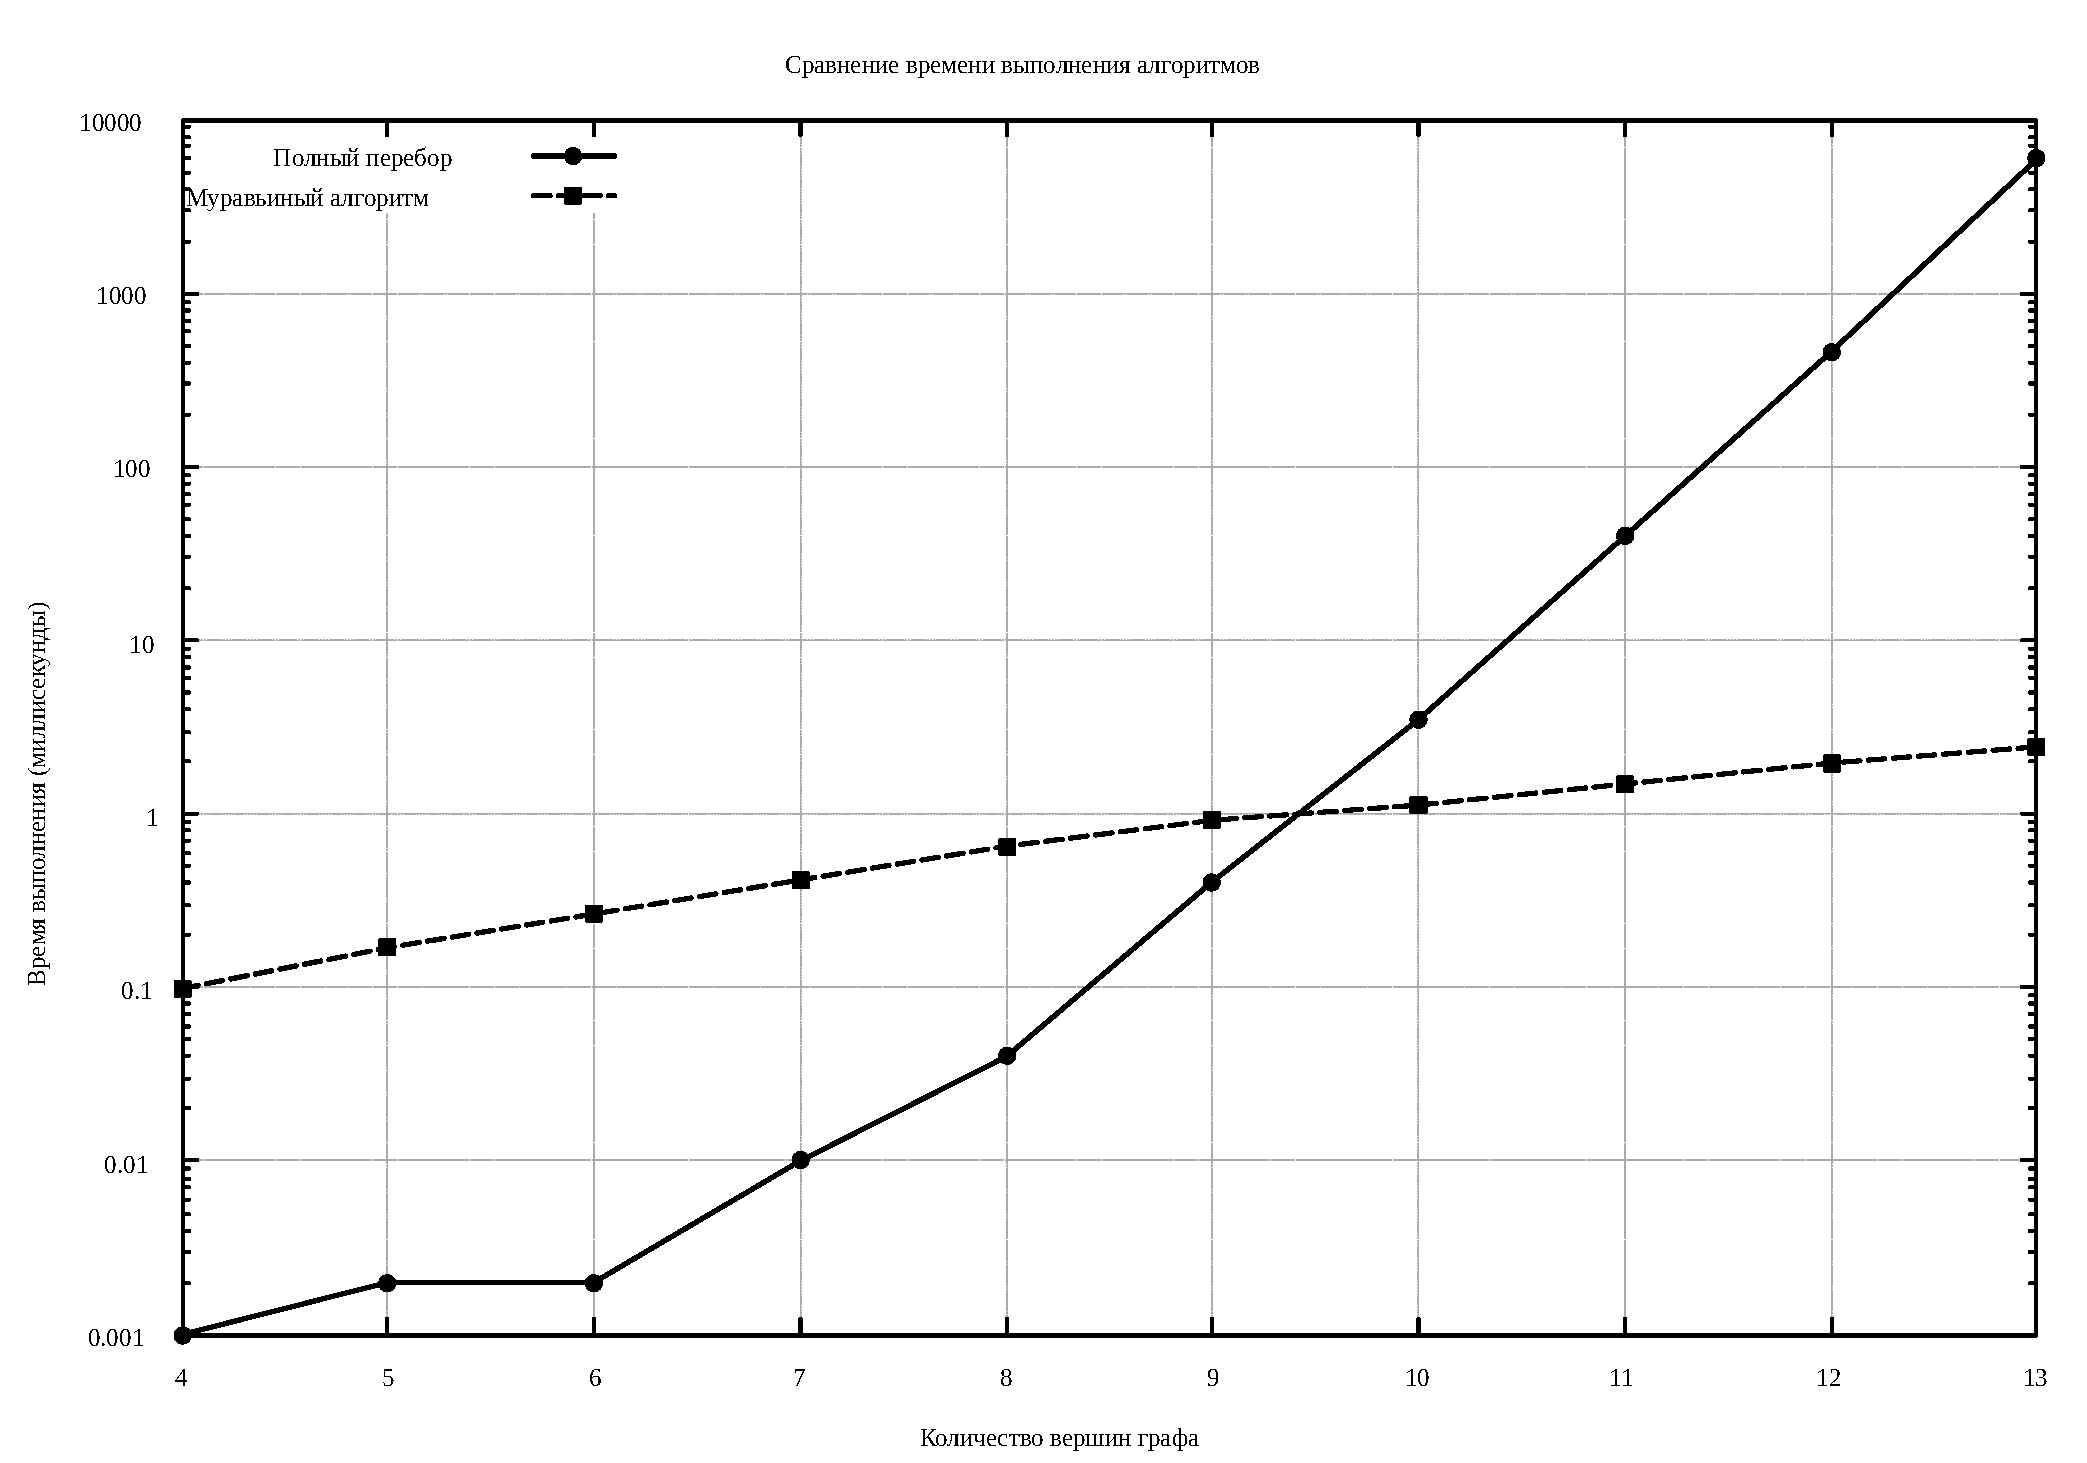
\includegraphics[width=1\textwidth]{images/zamer.pdf}
	\caption{Схема алгоритма решения задачи коммивояжёра часть 1}
	\label{fig:zamer}
\end{figure}

\clearpage

\section{Параметризация}

Для проведения параметризации муравьиного алгоритма были использованы три полносвязных графа,
каждый из которых содержит по 10 вершин. Веса рёбер представляют собой затраты времени на переход
между вершинами и находятся в диапазоне от 5 до 40 единиц. Такой выбор диапазона обеспечивает
сопоставимость результатов между графами и позволяет корректно оценивать поведение алгоритма.
Характеристики графов:

\begin{itemize}
	\item \textbf{граф 1}: 10 вершин, веса рёбер распределены в диапазоне 5---30. 
	Эталонная длина оптимального гамильтонова цикла 
	\(L^{(1)}_{\text{opt}} = 112\);
	
	\item \textbf{граф 2}: 10 вершин, веса рёбер распределены в диапазоне 10---35. 
	Эталонная длина оптимального гамильтонова цикла 
	\(L^{(2)}_{\text{opt}} = 128\);
	
	\item \textbf{граф 3}: 10 вершин, веса рёбер распределены в диапазоне 15---40. 
	Эталонная длина оптимального гамильтонова цикла 
	\(L^{(3)}_{\text{opt}} = 147\);
\end{itemize}

\subsection{Рекомендации по выбору параметров}

На основе проведённого анализа таблиц~\ref{tab:param-full-1} и~\ref{tab:param-full-2} можно дать следующие рекомендации по выбору параметров муравьиного алгоритма:

\begin{itemize}
    \item \textbf{параметр \(\alpha\) (влияние феромона)}: оптимальное значение \(\alpha = 0.5\). При меньших значениях (\(\alpha = 0.1, 0.2\)) алгоритм показывает нестабильные результаты, так как недостаточно учитывает накопленный опыт колонии. При больших значениях (\(\alpha > 1.0\)) алгоритм преждевременно сходится к субоптимальным решениям из-за чрезмерного влияния феромонов.
    
    \item \textbf{параметр \(\beta\) (влияние эвристики)}: оптимальные значения находятся в диапазоне \(3.0-5.0\). При \(\beta = 2.0\) наблюдается повышенная вероятность попадания в локальные оптимумы, особенно при высоких значениях коэффициента испарения. Значения \(\beta \geqslant 3.0\) обеспечивают лучший баланс между исследованием и эксплуатацией.
    
    \item \textbf{коэффициент испарения \(\rho\)}: оптимальные значения находятся в диапазоне \(0.2-0.5\). При \(\rho = 0.2\) алгоритм демонстрирует хорошую сходимость на всех тестовых графах. Значения \(\rho \geqslant 0.7\) приводят к чрезмерно быстрому испарению феромонов, что ухудшает качество решений, особенно на графах с большим разбросом весов рёбер.
\end{itemize}

Наиболее устойчивые результаты наблюдаются при следующих комбинациях параметров:
\begin{itemize}
    \item \(\alpha = 0.5\), \(\beta = 4.0\), \(\rho = 0.2-0.7\) (обеспечивает нулевое отклонение на всех тестовых графах)
    \item \(\alpha = 0.5\), \(\beta = 5.0\), \(\rho = 0.2-0.7\) (аналогично устойчивые результаты)
\end{itemize}



Для каждого набора параметров (\(\alpha\), \(\beta\), \(\rho\))
алгоритм запускался 10 раз на каждом графе.
В качестве метрики качества использовалось максимальное относительное отклонение
найденного маршрута от эталонного:
\[
\delta_{\max} = \max_i \frac{\lvert L_i - L_{\text{opt}} \rvert}{L_{\text{opt}}}.
\]

Результаты параметризации приведены в таблице~\ref{tab:param-full}.



\section{Вывод}

Проведённые замеры показали, что полный перебор обеспечивает точное
решение, однако его вычислительная сложность экспоненциально возрастает с
увеличением числа вершин. На малых графах время работы остаётся приемлемым,
но уже начиная с размеров $n \ge 10$ время выполнения резко увеличивается,
что подтверждается результатами.

Муравьиный алгоритм продемонстрировал значительно более стабильное время
выполнения при увеличении числа вершин. Хотя получаемые решения могут иметь
отклонение от оптимального значения, в рамках заданного ограничения по
времени маршрут, как правило, удаётся построить. Среднее отклонение оказалось
незначительным, а в ряде случаев алгоритм находил оптимальный цикл.

\clearpage
